\section{Mixture Models}
\paragraph{Soft Clustering}
The term Soft Clustering is ambiguous since it can refer to the algorithm or to the model:
\begin{description}
\item[Algorithmic:] Soft $K$-Means: Instead of assigning a point to exactly one cluster. Consider assigning a probability that a data point belongs to a certain cluster. 
\item[Model relaxation:] The model can be relaxed by replacing the "hard" constraint given by 
    \begin{align*}
        z_{k,n}\in \{0,1\}, \quad \sum_{k=1}^K z_{k,n} =1,
    \end{align*}
    and replace it by the \emph{soft constraint}:
    \begin{align*}
        z_{k,n} \in [0,1], \quad \sum_{k=1}^K z_{k,n} =1.
    \end{align*}
    This relaxed model \textbf{cannot} be written in Matrix factorisation form.
\end{description}

\subsection{Introduction}
The mixture of $K$ probability densities is defined as
\begin{align*}
    p(x) = \sum_{k=1}^K \pi_K p(x|\theta_k).
\end{align*}
Each probability distribution $p(x|\theta_k)$ is a \emph{component} of the mixture and has its own parameters $\theta_k$. Almost any continuous density can be approximated by using a sufficient number of component distributions. For a Gaussian component distribution the parameters $\theta_k$ are given by the mean $\mu_k$ and the covariance $\Sigma_k$. 


Mixture models are constructed from:
\begin{itemize}
    \item Component distributions of the form $p(x|\theta_k)$.
    \item Mixing coefficients $\pi_k$ that give the probability of each component.
\end{itemize}
In order for $p(x)$ to be a proper distribution, we have to ensure that
\begin{align*}
    \sum_{k=1}^K \pi_k=1\quad \text{and} \quad \pi_k \geq 0,\ 1\leq k\leq K.
\end{align*}
Therefore, the parameters $\pi_k$, $1\leq \leq K$ define a \emph{categorical} distribution which represents the probability of each component distribution.

\subsection{Gaussian Mixture Model}
The Gaussian Mixture Model (GMM) uses Gaussians as the component distributions. We thus assume the following distribution for our data:
\begin{align*}
    p(x) = \sum_{k=1}^K \pi_k \normal (x|\mu_k,\Sigma_k).
\end{align*}
Given data points $\{x_1,\ldots, x_N\}$, we then aim at learning parameters $\mu_k$, $\Sigma_k$, such that we approximate the data as closely as possible. This is equivalent to finding the parameters that \emph{maximise the likelihood} of the data.

\subsubsection{Generative Viewpoint}
Given the model parameters $\Sigma$, $\mu$, $\pi$, sample the data $x_n$ as follows:
\begin{enumerate}
    \item Sample a cluster index $k$ according to the probabilities $\pi_k$.
    \item Sample a data point $x_n$ from the distribution $p(x_n|\mu_k, \Sigma_k)$.
\end{enumerate}

\subsubsection{Parameter Estimation}
We assume that the data points $x_n$ are independent and identically distributed (i.i.d.). The probability or likelihood of the observed data $X$, given the parameters can thus be written as:
\begin{align*}
    p(X|\pi,\mu,\Sigma) = \prod_{n=1}^N p(x_n) = \prod_{n=1}^N\sum_{k=1}^K \pi_k \normal(x_n|\mu_k, \Sigma_k).
\end{align*}

We aim at finding the parameters that maximise the likelihood of the data:
\begin{align*}
(\hat \pi, \hat \mu, \hat \Sigma) \in \argmax_{\pi,\mu,\Sigma} p(X|\pi, \mu, \Sigma).
\end{align*}
To simplify the expression one takes the logarithm, such that the product becomes a sum:
\begin{align*}
(\hat \pi, \hat \mu, \hat \Sigma) \in \argmax_{\pi,\mu,\Sigma}\sum_{n=1}^N 
    \log \left\{ 
        \sum_{k=1}^K \pi_k \normal (x_n|\mu_k, \Sigma_k)
        \right\}.
\end{align*}
Due to the presence of the summation over $k$ inside the logarithm, the maximum likelihood solution for the parameters no longer has a closed-form analytic solution. In order to solve the equation we make use of an algorithmic approach: \emph{Expectation Maximisation}.

\subsubsection{Probability of assigning a data point to a cluster}
We use the Bayes' rule to get:
\begin{align*}
    \gamma(z_k) := p(z_k=1|x) &= {p(z_k=1)p(x|z_k=1) \over \sum_{j=1}^k p(z_j=1) p(x|z_j=1)}\\
     &= {\pi_k \normal(x|\mu_k, \Sigma_k)\over \sum_{j=1}^K \pi_j \normal(x|\mu_j, \Sigma_j)}.
\end{align*}
\subsubsection{Expectation-Maximisation for Gaussian Mixture Models}
A powerfule method for finding maximum likelihood solutions for models with latent variables. Setting the derivatives of $\log p(X|\pi, \mu, \Sigma)$ with respect to the means $\mu_k$ to zero, we obtain:
\begin{align*}
    0 = \sum_{n=1}^N \underbrace{\pi_k \normal(x_n|\mu_k, \Sigma_k) \over \Sigma_j \pi_j \normal(x_n|\mu_j, \Sigma_j)}_{\gamma(z_{k,n})} \Sigma_k^{-1} (x_n-\mu_k).
\end{align*}
Assume that $\Sigma_k$ is not singular. Multiplying by $\Sigma_k$ we obtain:
\begin{align*}
    \sigma_k &= {1\over N_k} \sum_{n=1}^N \gamma(z_{k,n})x_n,\\
    N_k &= \sum_{n=1}^N \gamma(z_{k,n}).
\end{align*}
The mean $\mu_k$ is obtained by taking a weighted mean of all the points in the data set.

Maximising $\log p(X|\pi, \mu, \Sigma)$ with respect to the mixing coefficients $\pi_k$ and taking account of the constraint which requires the mixing coefficients to sum to one, can be achieved using the following Lagrangian:
\begin{align*}
    \log p(X|\pi, \mu, \Sigma) + \lambda \left( \sum_{k=1}^K\pi_k-1\right),
\end{align*}
which gives 
\begin{align*}
    0 = \sum_{n=1}^N {\pi_k \normal(x_n|\mu_k, \Sigma_k) \over \Sigma_j \pi_j \normal(x_n|\mu_j, \Sigma_j)}+\lambda,\\
    \implies \pi_k = {N_k\over N}.
\end{align*}
Therefore, $\pi_k$ is given by the average responsibility of the $k$-th component.

\subsubsection{Algorithm}
Given a Gaussian mixture model, the goal is to maximise the likelihood function with respect to the parameters.
\begin{enumerate}
    \item Initialise the means $\mu_k$, and mixing coefficients $\pi_k$. Set the $\Sigma_k$ to the given covariances.
    \item \textbf{E-step}. Evaluate the responsibilities using the current parameter values:
        \begin{align*}
             \gamma(z_{k,n}) = {\pi_k \normal(x|\mu_k, \Sigma_k)\over \sum_{j=1}^K \pi_j \normal(x|\mu_j, \Sigma_j)}.
        \end{align*}
    \item \textbf{M-step}. Re-estimate the parameters using the current responsibilities
        \begin{align*}
            \mu_k^{new} &= {1\over N_k} \sum_{n=1}^N \gamma(z_{k,n}) x_n,\\
            \Sigma_k^{new} &= {1\over N_k} \sum_{i=1}^N \gamma(z_{k,n})\cdot (x_i-\mu_k^{new})(x_i-\mu_k^{new})^T &1\leq k \leq K,\\
            \pi_k^{new} &= {N_k\over N} \qquad\text{where } N_k = \sum_{n=1}^N \gamma(z_{k,n}).
        \end{align*}
    \item Evaluate the log likelihood and check for convergence of either the parameters or the log likelihood.
\end{enumerate}

\subsubsection{Relation to $K$-means}
The EM algorithm makes a soft assignment based on posterior probabilities\footnote{The posterior probability is the probability of the parameters $\theta$ given the evidence $X: p(\theta|X)$ (Wikipedia)}. Whereas the $K$-means algorithm performs a hard assignment of data points to clusters.

The $K$-means algorithm does not estimate the covariances of the clusters but only the cluster means. The EM algorithm can be reduced to $K$-means.

The EM algorithm takes more iterations to converge than $K$-means.

The $K$-means algorithm can be used to find a suitable initialisation for a Gaussian mixture model.

There will generally be multiple local maxima of the log likelihood function, and EM is not guaranteed to find the largest of these maxima.

\subsubsection{Log Likelihood}
\begin{align*}
    \mathbb E_Z[\log p(X,Z| \mu,\Sigma, \pi)] \rightarrow - {1\over 2} \sum_{n=1}^N\sum_{k=1}^K z_{k,n} \norm{x_n-\mu_k}_2^2 + \text{ const}.
\end{align*}


\subsubsection{Matrix Factorisation}
Assumption: $z_{k,n} \in [0,1]$ and $\sum_{k=1}^K z_{k,n} = 1 \ \forall n$.
\begin{align*}
    \norm{X-UZ}_F^2 &= \sum_{n=1}^N \norm{x_n \sum_{k=1}^K z_{k,n}u_k}_2^2 \\
        &= \sum_{n=1}^N \left( \norm{x_n}^2 -2 \sum_{k=1}^K x_n u_k z_{k,n} + \left( \sum_{k=1}^K z_{k,n}u_k \right)\right)\\
        &= \sum_{n=1}^N\sum_{k=1}^K z_{k,n}\norm{x_n-u_k}_2^2 
            - \sum_{n=1}^N\sum_{k=1}^K z_{k,n} \left( u_k-\sum_{k'=1}^K z_{k',n}u_{k'}\right)^2
\end{align*}

For identity covariance matrices GMM gives an upper bound!

\section{Model Order Selection and Information Criteria}
The selection of the number of clusters is a trade-off between two conflicting goals:
\begin{description}
    \item[Data Fit:] We want to predict the data well, e.g., maximises the likelihood. The likelihood usually increases by increasing the clusters.
    \item[Complexity:] Choose a model that abstracts a lot of data. This is often measured by the number of free parameters.
\end{description}

\subsubsection{Negative Log-Likelihood}
The smaller the negative log-likelihood, the better the fit.
\begin{align*}
    -\log p(X|\pi, \mu, \Sigma) = - \sum_{n=1}^N \log \left\{ \sum_{k=1}^K \pi_k \normal(x_n|\mu_k, \Sigma_k)\right\}
\end{align*}
In practice increasing K does not always decrease the negative log-likelihood due to local minima.\begin{figure}[H]
    \centering
    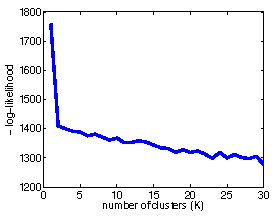
\includegraphics[width=0.5\textwidth]{img/kmeans_log_likelihood_plot}
\end{figure}

\subsection{AIC and BIC}
Achieve balance between data fit (measured by likelihood $p(X|.)$) and complexity. Complexity can be measured by the number of free parameters $\kappa(\cdot)$.
\subsubsection{AIC - Akaike Information Criterion}
\begin{align*}
    AIC(U,Z|x_1,\ldots, x_N) = -\log(p(X|.)+\kappa(U,Z)
\end{align*}

\subsubsection{BIC - Bayesian Information Criterion}
\begin{align*}
    BIC(U,Z|x_1,\ldots, x_N) = -\log(p(X|.)+{1\over 2}\kappa(U,Z)\log N
\end{align*}

Generally speaking, the BIC criterion penalises complexity more
than the AIC criterion.

A single AIC (BIC) result is meaningless. One has to repeat the analysis for different Ks and compare the differences: the most suitable number of clusters corresponds to the smallest AIC (BIC) value.

\paragraph{Example} Mixture of Gaussians with fixed covariance. NUmber of free parameters:
\begin{align*}
    \kappa(U,Z) = K\cdot D+(K-1).
\end{align*}

\begin{figure}[H]
    \centering
    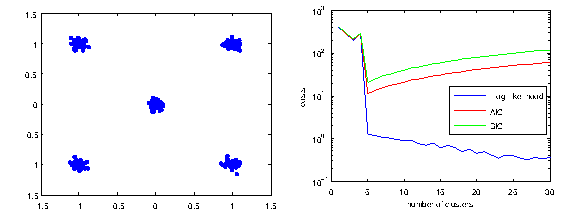
\includegraphics[width=\textwidth]{img/kmeans_cluster_comparison}
    \caption{Comparison of AIC, BIC and negative Log-Likelihood an a synthetic dataset with $5$ clusters.}
\end{figure}

